\subsection{插件登录 ECNU 及辅助登录}\label{subsec:plugin-login-ecnu}

插件许多功能需要调用 ECNU 提供的各种接口。
接口的调用依赖于 ECNU 各个系统的登录缓存(在项目内部保存为 \verb`LoginCache`)。
为了获取有效的登录缓存简化登录操作,
插件登录使用了 WebDriver 控制浏览器实现自动化或半自动化的辅助登录流程。

在插件登录时,会出现浏览器 ECNU 统一身份认证的界面,登录有两种方式。
\begin{itemize}
    \item 方法一:填写图\ref{fig:uia-login-form} 中的表单实现登录。
    \item 方法二:扫描图\ref{fig:uia-login-qrcode} 中的二维码实现登录。
\end{itemize}

\begin{table}[H]
    \centering
    \begin{tabular}{cc}
        \begin{minipage}[H]{0.5\textwidth}
            \centering
            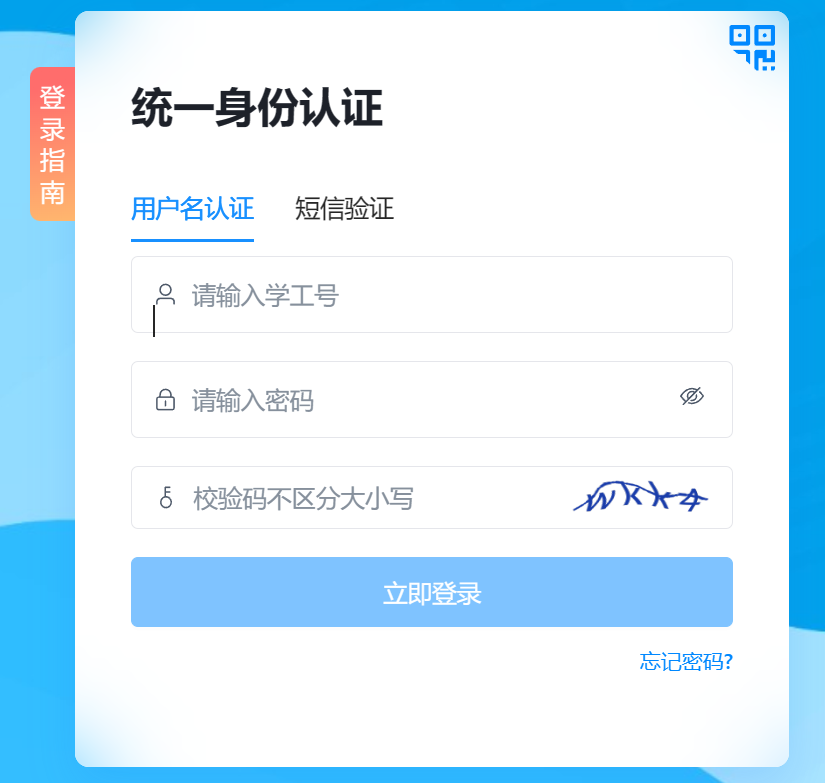
\includegraphics[width=0.8\textwidth]{img/uia_login_form}
            \captionof{figure}{ECNU UIA 登录界面(表单)}
            \label{fig:uia-login-form}
        \end{minipage} &
        \begin{minipage}[H]{0.5\textwidth}
            \centering
            
\includegraphics[width=0.8\textwidth]{img/uia_login_qrcode}
            \captionof{figure}{ECNU UIA 登录界面(二维码)}
            \label{fig:uia-login-qrcode}
        \end{minipage}
    \end{tabular}
\end{table}

\begin{rmr}[切换表单登录和二维码登录]
    \quad 表单登录:
    可以在项目根目录创建文件 \verb`login_info.toml`
    然后填写如下内容(替换尖括号以内的部分)。
    插件登录时会读取此文件中的学号密码,自动填写图\ref{fig:uia-login-form} 中的表单,实现全自动辅助登录。
    % @formatter:off
    \begin{verbatim}
stu_number = "<填写学号>"
password = "<填写数据库密码>" \end{verbatim}
    % @formatter:on

    \quad 二维码登录:
    删除 \verb`login_info.toml` 文件,
    此时插件辅助登录时会截取二维码图片并发送至邮箱提醒(如果已配置 \verb`email_notifier` 插件,见\ref{plugin-email-notifier})。 % todo 完成这个插件的介绍
    可以使用微信扫描二维码或用微信打开邮件中的连接实现半自动登录。
\end{rmr}

\subsubsection{辅助登录大致实现}

当此软件执行辅助登录的时候:

\begin{description}
    \item[二维码登录]
    进入 ECNU 统一身份认证(下面简称 UIA)界面之后,辅助登录默认使用二维码登录而不是表单登录。
    二维码登录时,脚本截取 UIA 二维码登录图片然后发送到目标邮箱,通过用户微信扫描二维码或者微信打开邮箱中的连接来实现登录。
    \item[表单登录]
    如果创建了 \verb`login_info.toml` 文件(步骤见上述提示),那么脚本会读取其中的学号和密码并自动填写到 UIA 表单中。
    表单中的验证码通过开源库 \hyperref{https://github.com/sml2h3/ddddocr}{DDDDocr} 来识别,成功识别四位验证码之后模拟点击登录按钮来登录。
    如果验证码识别失败则刷新重试。
\end{description}

成功登录 UIA 之后,各个插件通过自己实现的缓存抓取函数(\textit{Cache Grabber})在各个 ECNU 系统中获得所需要的登录缓存。

最终,登录缓存通过插件加载器(\textit{Plugin Loader})分发给各个插件。